\documentclass[10pt,twocolumn,letterpaper]{article}

\usepackage{cvpr}
\usepackage{times}
\usepackage{epsfig}
\usepackage{graphicx}

\usepackage{booktabs}
\usepackage{xspace}

%\usepackage{algorithm}
%\usepackage{algorithmic}
%\usepackage{hyperref}
%\usepackage{url}
%\newcommand{\theHalgorithm}{\arabic{algorithm}}
%
%\usepackage{latexsym}
%\usepackage{amsmath,amsfonts}
%\usepackage{amssymb}
%\usepackage{amsthm}
%\usepackage{relsize}
%\usepackage{mathtools}
%\usepackage{tikz}
%\usepackage{array}
%\usepackage{subcaption}
%\usepackage{comment}
%\usepackage{multirow}
%\usepackage{aliascnt}
%\usepackage{xspace}
%\usepackage[bb=fourier]{mathalfa}
%%\usepackage[font=small]{caption}
%\usepackage{siunitx}
%\usepackage{tablefootnote}
%\usepackage{multirow}
%\usepackage{microtype}
%\usepackage[export]{adjustbox}
%\usepackage{footmisc}

% Add a period to the end of an abbreviation unless there's one
 \makeatletter
 \DeclareRobustCommand\onedot{\futurelet\@let@token\@onedot}
 \def\@onedot{\ifx\@let@token.\else.\null\fi\xspace}
 \def\eg{e.g\onedot} \def\Eg{E.g\onedot}
 \def\ie{i.e\onedot} \def\Ie{I.e\onedot}
 \def\cf{cf\onedot} \def\Cf{Cf\onedot}
 \def\etc{etc\onedot} \def\vs{vs\onedot}
 \def\wrt{w.r.t\onedot} \def\dof{d.o.f\onedot}
 \def\etal{\textit{et~al\onedot}} \def\iid{i.i.d\onedot}
 \def\Fig{Fig\onedot} \def\Eqn{Eqn\onedot} \def\Sec{Sec\onedot}
 \def\vs{vs\onedot}
 \makeatother


\DeclareRobustCommand{\figref}[1]{Figure~\ref{#1}}
\DeclareRobustCommand{\figsref}[1]{Figures~\ref{#1}}

\DeclareRobustCommand{\Figref}[1]{Figure~\ref{#1}}
\DeclareRobustCommand{\Figsref}[1]{Figures~\ref{#1}}

\DeclareRobustCommand{\Secref}[1]{Section~\ref{#1}}
\DeclareRobustCommand{\secref}[1]{Section~\ref{#1}}

\DeclareRobustCommand{\Secsref}[1]{Sections~\ref{#1}}
\DeclareRobustCommand{\secsref}[1]{Sections~\ref{#1}}

\DeclareRobustCommand{\Tableref}[1]{Table~\ref{#1}}
\DeclareRobustCommand{\tableref}[1]{Table~\ref{#1}}

\DeclareRobustCommand{\Tablesref}[1]{Tables~\ref{#1}}
\DeclareRobustCommand{\tablesref}[1]{Tables~\ref{#1}}

\DeclareRobustCommand{\eqnref}[1]{Equation~(\ref{#1})}
\DeclareRobustCommand{\Eqnref}[1]{Equation~(\ref{#1})}

\DeclareRobustCommand{\eqnsref}[1]{Equations~(\ref{#1})}
\DeclareRobustCommand{\Eqnsref}[1]{Equations~(\ref{#1})}

\DeclareRobustCommand{\chapref}[1]{Chapter~\ref{#1}}
\DeclareRobustCommand{\Chapref}[1]{Chapter~\ref{#1}}

\DeclareRobustCommand{\chapsref}[1]{Chapters~\ref{#1}}
\DeclareRobustCommand{\Chapsref}[1]{Chapters~\ref{#1}}


% \setlength{\topskip}{0mm}
% \setlength{\abovecaptionskip}{3mm}
% \setlength{\belowcaptionskip}{3mm}
% \setlength{\textfloatsep}{5mm}

\hyphenation{po-si-tive}
% Include other packages here, before hyperref.

% If you comment hyperref and then uncomment it, you should delete
% egpaper.aux before re-running latex.  (Or just hit 'q' on the first latex
% run, let it finish, and you should be clear).
\usepackage[pagebackref=true,breaklinks=true,letterpaper=true,colorlinks,bookmarks=false]{hyperref}

% \cvprfinalcopy % *** Uncomment this line for the final submission

\def\cvprPaperID{****} % *** Enter the CVPR Paper ID here
\def\httilde{\mbox{\tt\raisebox{-.5ex}{\symbol{126}}}}

% Pages are numbered in submission mode, and unnumbered in camera-ready
\ifcvprfinal\pagestyle{empty}\fi
\begin{document}

\newcommand{\nmn}{Neural Module Networks\xspace}
\newcommand{\mod}[1]{{\small\texttt{#1}}}
\newcommand{\todo}{\textcolor{red}}
\newcommand{\shapes}{{\textsc{shapes}\xspace}}
\newcommand{\marcus}[1]{\textcolor{blue}{Marcus: #1}}
%%%%%%%%% TITLE
\title{Deep Compositional Question Answering with Neural Module Networks}

\author{First Author\\
Institution1\\
Institution1 address\\
{\tt\small firstauthor@i1.org}
% For a paper whose authors are all at the same institution,
% omit the following lines up until the closing ``}''.
% Additional authors and addresses can be added with ``\and'',
% just like the second author.
% To save space, use either the email address or home page, not both
\and
Second Author\\
Institution2\\
First line of institution2 address\\
{\tt\small secondauthor@i2.org}
}

\maketitle
%\thispagestyle{empty}

%%%%%%%%% ABSTRACT
\begin{abstract}
  Visual question answering differs from many other vision tasks in that the
  computational structure necessary to produce an answer is not fixed, but
  instead varies depending on the question. \marcus{I am confused with this sentence. It is stated like known fact, but prior work says differently\ldots and that what we want to show in the paper.} 
  At the same time, the task is
  fundamentally compositional in nature---answering a question like \emph{where
  is the dog?} shares substructure with questions like \emph{what color is the
  dog?} and \emph{where is the cat?}. This paper seeks to simultaneously exploit the
  representational capacity of deep networks and the dynamic compositional
  structure of questions.  We describe a procedure for constructing and learning
  \emph{neural module networks}, which compose collections of jointly-trained
  neural ``modules'' into deep networks for question answering. Our approach
  decomposes questions into their linguistic substructures, and uses these
  structures to dynamically instantiate modular networks (with reusable
  components for recognizing dogs, classifying colors, etc.). The resulting
  compound networks are jointly trained. We evaluate our approach on three
  challenging datasets for visual question answering, achieving several
  state-of-the-art results.
%Answering a question about an image, is a challenging task which requires understanding the question, grounding it in the image and jointly reasoning about the image content to produce a correct answer. Intuitively, this task is compositional in nature, \ie answering \emph{where the dog} in an image is can partially share an representation with \emph{which color the dog} is or \emph{where the cat} is. On the other hand, learning deep neural networks has shown impressive progress in question answering and related tasks. Consequently, we propose \emph{\nmn}, which composes several, jointly trained neural modules to answer questions about images. Specifically our approaches decomposes questions into their linguistic substructures and instantiates corresponding neural ``modules'' (\eg \emph{where, which color, dog}) which are stacked to a deep network. The resulting compound
%  networks are then jointly trained, whose composable neural ``modules'' 
%  can be dynamically remixed to interpret also novel questions. We evaluate our approach
%  on three challenging datasets for visual question answering, achieving
%   overall state-of-the-art performance, but outperforming related work for more complex questions.
\end{abstract}

\section{Introduction} 

\begin{figure}[t] \begin{center}
    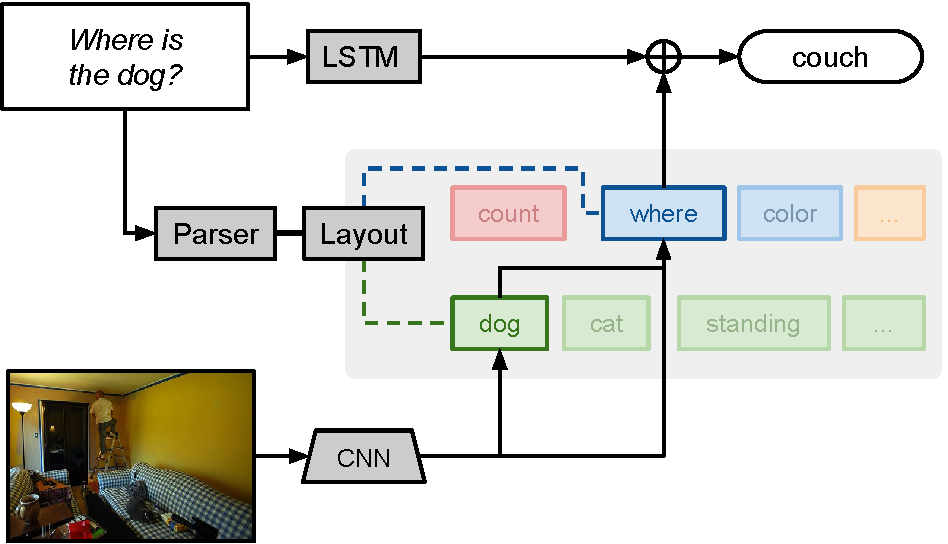
\includegraphics[width=\linewidth]{fig/teaser} \end{center} \caption{
      A schematic representation of our proposed model---the shaded gray area is a
      {\it neural module network} of the kind introduced in this paper. Our
      approach uses a natural language parser to dynamically lay out a deep
      network composed of reusable modules. For visual question answering tasks,
      an additional sequence model provides sentence context and learns
      common-sense knowledge.
    } \label{fig:teaser}
\end{figure}

This paper describes \emph{neural module networks} (NMNs), a modular framework
for visual quesiton answering. We answer natural language questions about images
using collections of jointly-trained neural ``modules'', dynamically assembled
into deep networks based on linguistic structure. 

The visual QA task has been the subject of a great deal of recent research
attention
\cite{antol15iccv,gao2015you,ma15arxiv,malinowski15iccv,ren2015image,yu15arxiv},
and has significant applications to human-robot interaction, search, and
accessibility.  Visual QA requires sophisticated understanding of both visual
scenes and natural language.
%
Concretely, given an image and an associated question (e.g.\ \emph{where is
the dog?}), we wish to predict a corresponding answer (e.g.\ \emph{on the
couch}, or perhaps just \emph{couch}). Recent successful approaches represent
questions as bags of words, or encode in the question using a recurrent neural
network \cite{malinowski15iccv} and train a simple classifier on the encoded
question and image. In contrast to these monolithic approaches, another line of
work for textual QA \cite{Liang13DCS} and image QA \cite{malinowski14nips} uses
semantic parsers to decompose questions into logical expressions. These logical
expressions are evaluated against a purely logical representation of the world,
which may be provided directly or extracted from an image
\cite{Krish2013Grounded}.

In this paper we draw from both lines of research, presenting a technique for
integrating the representational power of neural networks with the flexible
compositional structure afforded by symbolic approaches to semantics.  Rather
than relying on a monolithic network structure to answer all questions, our
approach assembles a network on the fly from a collection of specialized,
jointly-learned modules (\autoref{fig:teaser}). Rather than reasoning over
truth values, we remain entirely in the domain of visual features and
attentions.

Our approach first analyzes
each question with an off-the-shelf semantic parser, and uses this analysis to
determine the basic computational units (attention, classification, etc.) needed
to answer the question, as well as the relationships between the modules. In
\autoref{fig:teaser}, we first produce an attention focused on the dog, which
passes its output to
a location classifier. Depending on the underlying structure, these messages
passed between modules may be raw image features, attentions, or classification
decisions; each module is determined by its input and output types.
Different kinds of modules are shown in different colors; attention modules
(like \mod{dog}) are shown in green, while labeling modules (like
\mod{where}) are shown in blue.
%Different kinds of modules are marked with different
%colors in \Figref{fig:teaser}: for example the \mod{attend[$dog$]} module
%(green) produces a spatial heatmap while the \mod{classify[$where$]} (blue)
%recognizes what is in the image region localized by the attention heatmap.
Importantly, all modules of a NMN are independent and composable, which allows
the computation to be different for each problem instance, and possibly
unobserved during training. 
%So that we can answer novel question at test time, such as
%\emph{Where is the banana?}, even we only saw \emph{count} or
%\emph{color} question about \emph{bananas} during training.  
Outside the NMN, our final answer incorporates the image scene knowledge
(using a full frame CNN) and uses a recurrent network (LSTM) to read the
question, which has been shown to be important to model common sense knowledge
and dataset biases \cite{malinowski15iccv}.

%Where previous work has
%treated both the image and the question as inputs to a monolithic
%classification model, we instead take the perspective that a question is a
%noisy specification of a hidden computation that must be performed on the image
%to produce an answer. Crucially, this computation may be different for each
%problem instance, and is never observed observed during training.

%Our approach bears a superficial resemblance to a classical semantic parser.
%However, instead of mapping from questions to logical forms, our model maps
%from questions to neural network structures. These networks are assembled on
%the fly (possibly into novel topologies) from a collection of jointly-learned
%neural ``modules''. Finally, they are evaluated against the input image to
%produce an answer.




%This paper presents a technique for following natural language instructions
%(and performing other dynamically-specified tasks) by assembling deep neural
%networks on the fly from an inventory of pre-trained components.

We evaluate our approach on three visual question answering tasks. On the
recently-released CocoQA \cite{yu15arxiv} and VQA \cite{antol15iccv} datasets,
we achieve results comparable to or better than existing approaches, and show
that our approach specifically outperforms previous work on questions with
compositional structure (\eg requiring that an object be located and one of its
attributes described). It turns out, however, that many of the questions in both
datasets are quite simple, with little composition or reasoning required. To
test our approach's ability to handle harder questions, we introduce
a new dataset of synthetic images paired with complex questions involving
spatial relations, set-theoretic reasoning, and shape and attribute recognition.
On this dataset we outperform competing approaches by as much as 25\% absolute
aaccuracy.

While all the applications considered in this paper involve visual question
answering, the general architecture is potentially of broader usefulness, and
might be more generally applied to visual referring expression resolution (XXX)
or question answering about natural language texts (XXX).

%We evaluate our approach on two visual question answering tasks. First we
%present a new synthetic image dataset paired with a complex set of queries
%(involving spatial relations, logical operators, and shape and attribute
%recognition). Next, we consider a hard subset of the Microsoft VQA corpus of
%questions about natural images. In each case, an NMN-based approach outperforms
%state-of-the-art models with more conventional recurrent architectures. We
%observe in particular that NMNs are able to make considerably better use of
%small training sets.

To summarize our contributions: We first describe neural module networks, a
general architecture for discretely composing heterogeneous, jointly-trained
neural modules into deep networks. Next, for the visual QA task specifically, we
show how to construct NMNs based on the output of a semantic parser, and use
these to successfully complete established visual question answering tasks.
Finally, we introduce a new dataset of challenging, highly compositional
questions about abstract shapes, and show that our model again outperforms
previous approaches. We will release this dataset, as well as code for all
systems described in this paper, upon publication.

\section{Motivations}

%Many tasks in computer vision, including recognition, detection, and captioning,
%share common substructure. For example, we might schematically express the
%sequence of computations performed by a recognizer as
%\begin{flushleft}
%  \mod{classify(pickMostRelevant(detectObjects))}
%\end{flushleft}
%or a detector as
%\begin{flushleft}
%  \mod{drawBoundaries(detectObjects)}
%\end{flushleft}
%
%In practice the picture is not this clean---classification or detection is
%performed end-to-end by a single neural network, and the boundaries between
%these ``phases'' are not clearly defined. Nevertheless we might expect \textit{a
%priori} that a network used for classification might expose intermediate
%representations useful for building a detector. 
We begin with two simple observations. First, that there is no single ``best
network'' for all purposes---state-of-the-art performance on the full range of
computer vision tasks that are studied requires a variety of different deep
network topologies. Second, though different networks are used for different
purposes, it is commonplace to initialize systems for many of vision tasks with
a prefix of a network trained for classification \cite{Long14FullyConvolutional} XXX. 
This has been shown to substantially reduce training time and improve accuracy. 

So while network structures are not \emph{universal} (in the sense that the same
network is appropriate for all problems), they are at least empirically
\emph{modular} (in the sense that intermediate representations for one task are
useful for many others). 

Can we generalize this idea in a way that is useful for question answering?
Rather than thinking of question answering as a problem of learning a single
function to map from questions and contexts to answers, it's perhaps useful to
think of it as a highly-multitask learning setting, where each problem instance
is associated with a novel task, and the identity of that task is expressed only
noisily in language. In particular, where a simple question like \emph{is this a
truck?} requires us to retrieve only one piece of information from an image,
more complicated questions, like \emph{how many objects are to the left of
the toaster?} might require multiple processing steps. The compositional nature
of language (XXX) means that the number of such processing such steps is
potentially unbounded. Moreover, multiple \emph{kinds} of processing might be
required---repeated convolutions might identify a truck, but some kind of
recurrent architecture is likely necessary to count up to arbitrary numbers.

Thus our goal in this paper is to specify a framework for modular, composable,
jointly-trained neural networks. In this framework, we first predict the
structure of the computation needed to answer each question individually, then
realize this structure by constructing an appropriately-shaped neural network
from an inventory of reusable modules. These modules are learned jointly, rather
than trained in isolation, and specialization to individual tasks (identifying
properties, spatial relations, etc.) arises naturally from the training
objective.

%If we consider a few examples of questions:
%XXX
%\begin{center}
%  \begin{tabular}{ll}
%    {\it how many black cats?} & \mod{count(and(detect[cat], detect[black]))} \\
%    {\it what color is the cat?} & \mod{classify[color](detect[cat])} \\
%    {\it what color is the dog?} & \mod{classify[color](detect[dog])} \\
%    {\it is there a dog?} & \mod{exists(detect[dog])}
%  \end{tabular}
%\end{center}
%we again see that there is common computational substructure involved in solving
%the associated tasks.  With sub-networks for computing \mod{detect[cat]},
%\mod{classify}, \mod{count}, etc., we can in principle answer
%questions with novel structure like---e.g.\ {\it is there a black
%dog?}---without any additional training data.
%
%Note in particular that we expect these modules to differ not only in their
%parameters, but more fundamentally in their topologies. Intuitively,
%\mod{detect[cat]} should take an image as input, perform some
%fully-convolutional operation, and output an attention (understood as a
%distribution over positions in the image), while {\small\tt classify[color]}
%should take both the input image and such an attention, and map to a
%distribution over labels. Some computations require convolutional operations,
%some require fully-connected operations, and some (like counting) may require
%recurrent network structures. We should not expect that we will be able to use
%the same network layout for every problem, but do expect that parts of these
%networks may be reused in different orders.


\section{Motivations}

Many tasks in computer vision, including recognition, detection, and captioning,
share common substructure. For example, we might schematically express the
sequence of computations performed by a recognizer as
\begin{flushleft}
  \mod{classify(pickMostRelevant(detectObjects))}
\end{flushleft}
or a detector as
\begin{flushleft}
  \mod{drawBoundaries(detectObjects)}
\end{flushleft}

In practice the picture is not this clean---classification or detection is
performed end-to-end by a single neural network, and the boundaries between
these ``phases'' are not clearly defined. Nevertheless we might expect \textit{a
priori} that a network used for classification might expose intermediate
representations useful for building a detector. Indeed, it is now commonplace to
initialize systems for a variety of vision tasks with a prefix of a network
trained for classification \cite{Long14FullyConvolutional}. This has been shown
to substantially reduce training time and improve accuracy. So while network
structures are not \emph{universal} (in the sense that the same network is
appropriate for all problems), they are at least empirically \emph{modular} (in
the sense that intermediate representations for one task are useful for many
others). 

Can we generalize this idea in a way that is useful for question answering?
Rather than thinking of question answering as a problem of learning a single
function to map from questions and contexts to answers, it's perhaps useful to
think of it as a highly-multitask learning setting, where each problem instance
is associated with a novel task, and the identity of that task is expressed only
noisily in language. If we consider a few examples of questions:
XXX
%\begin{center}
%  \begin{tabular}{ll}
%    {\it how many black cats?} & \mod{count(and(detect[cat], detect[black]))} \\
%    {\it what color is the cat?} & \mod{classify[color](detect[cat])} \\
%    {\it what color is the dog?} & \mod{classify[color](detect[dog])} \\
%    {\it is there a dog?} & \mod{exists(detect[dog])}
%  \end{tabular}
%\end{center}
we again see that there is common computational substructure involved in solving
the associated tasks.  With sub-networks for computing \mod{detect[cat]},
\mod{classify}, \mod{count}, etc., we can in principle answer
questions with novel structure like---e.g.\ {\it is there a black
dog?}---without any additional training data.

Note in particular that we expect these modules to differ not only in their
parameters, but more fundamentally in their topologies. Intuitively,
\mod{detect[cat]} should take an image as input, perform some
fully-convolutional operation, and output an attention (understood as a
distribution over positions in the image), while {\small\tt classify[color]}
should take both the input image and such an attention, and map to a
distribution over labels. Some computations require convolutional operations,
some require fully-connected operations, and some (like counting) may require
recurrent network structures. We should not expect that we will be able to use
the same network layout for every problem, but do expect that parts of these
networks may be reused in different orders.

Thus our goal in this paper is to specify a framework for modular, composable,
jointly-trained neural networks. In this framework, we first predict the
structure of the computation needed to answer each question individually, then
realize this structure by constructing an appropriately-shaped neural network
from an inventory of reusable modules. These modules are learned jointly, rather
than trained in isolation, and specialization to individual tasks (identifying
properties, spatial relations, etc.) arises naturally from the training
objective.

\section{Related work}

The idea of selecting a different network graph for each input datum is fundamental to both recurrent networks (where the network grows in the length of the input) \cite{Elman90RNN} and recursive neural networks (where the network is built, e.g., according to the syntactic structure of the input) \cite{Socher13CVG}. But both of these approaches ultimately involve repeated application of a single computational module (\eg an LSTM \cite{} or GRU \cite{} cell). Our basic contribution is in allowing the nodes of this graph to perform heterogeneous computations, and for "messages" of different kinds---raw image features, attentions, classification predictions---to be passed from one module to the next. We are unaware of any previous work allowing such mixed collections of modules to be trained jointly. 

\paragraph{non-image QA}
text only based: \cite{berant14acl,Liang13DCS}

\cite{geman15nas} a binary (yes/no) version of Visual Turing Test on synthetic data.

We are also unaware of past use of a semantic parser to predict network structures, or more generally to exploit the natural similarity between set-theoretic approaches to classical semantic parsing and attentional approaches to computer vision. As noted above, there is a large literature on learning to answer questions about structured knowledge representations from question--answer pairs, both with and without learning of meanings for simple predicates \cite{Liang13DCS,Krish2013Grounded}.

``neural'': \cite{iyyer14emnlp,weston14arxiv}

\paragraph{Grounding in images}
Deep Fragments \cite{karpathy14nips}, Flickr30k Entities \cite{plummer15iccv}.
Deep Visual-Semantic Alignments for Generating Image Descriptions \cite{karpathy15cvpr}.
(Image Retrieval using Scene Graphs \cite{johnson15cvpr})

\cite{Krish2013Grounded,matuszek12icml,kong14cvpr}

\paragraph{Datasets}
The present work is made possible by a number of recently-created corpora for question answering about images, including the DAQUAR dataset \cite{malinowski14nips}, the CocoQA dataset \cite{yu15arxiv}, and the VQA dataset \cite{antol15iccv}. 




\paragraph{image QA}
``classical'': \cite{malinowski14nips}

``neural'':
Several models for visual questioning have already been proposed in the literature \cite{ren2015image,ma15arxiv,gao2015you}, all of which use standard deep sequence modeling machinery to construct a joint embedding of image and text, which is immediately mapped to a distribution over answers. Here we attempt to more XXXly model the computational process needed to produce each answer, but also benefit from sequence and image embeddings XXX.

\section{Model}

Given a pre-trained \emph{network layout predictor} $P$, each training datum for
this task can be thought of as a 4-tuple $(w, p, x, y)$, where
\begin{itemize}
  \setlength\itemsep{0em}
  \item $w$ is a natural-language question
  \item $p = P(w)$ a network layout
  \item $x$ is an image
  \item $y$ is an answer
\end{itemize}
A model is fully specified by a collection of modules $\{ m \}$, each with
associated parameters $\theta_m$. Given $(w, p, x)$ as above, the model
instantiates a network according to $p$, passes $w$ and $x$ as inputs, and
obtains a distribution over labels (for the VQA task, we require the root module
to be a classifier). Thus a model corresponds to a predictive distribution $p(y\
|\ w, p, x; \theta)$.

In the remainder of this section, we first describe the set of modules used for
the VQA task, then explain the process by which questions are converted to
network layouts.

\subsection{Modules}

Our goal in this section is to identify a small set of modules that can be
assembled into all the configurations necessary for our tasks. This corresponds
to identifying a minimal set of composable vision primitives. The modules
operate on three basic data types: images, unnormalized attentions, and labels.
For the particular task and modules described in this paper, almost all
interesting compositional phenomena occur in the space of attentions, and it is
not unreasonable to characterize our contribution more narrowly as an
``attention-composition'' network. Nevertheless, other types may be
required in the future (for different new or for greater coverage in the VQA
domain).

\pagebreak
\paragraph{Attend}

An attention module \mod{attend[$x$]} convolves every position in the input
image with a weight vector (distinct for each $x$) to produce a heatmap or
unnormalized attention. So, for example, the output of the module {\small\tt
attend[dog]} is a matrix whose entries should be in regions of the image
containing cats, and small everywhere else, as shown below.\\
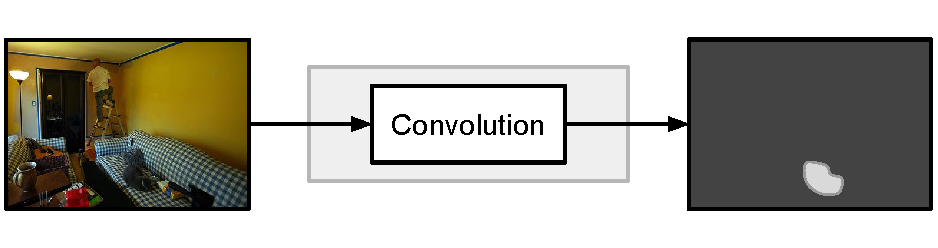
\includegraphics[width=\columnwidth]{fig/attend}

\paragraph{Re-attend}

A re-attention module \mod{re-attend[$x$]} performs a fully-connected mapping
from one attention to another. Again, the weights for this mapping are distinct
for each $x$. So \mod{re-attend[above]} should take an attention and shift the
regions of greatest activation upward (as below), while \mod{re-attend[not]}
should move attention away from the active regions.\\%[1em]
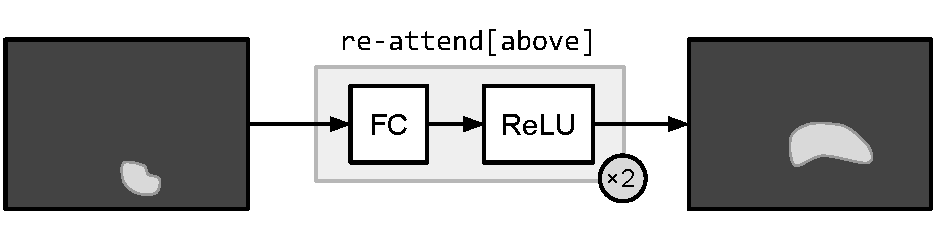
\includegraphics[width=\columnwidth]{fig/re-attend}

\paragraph{Combine}

A combination module \mod{combine[$x$]} merges two attentions into a single
attention. For example, {\small\tt combine[and]} should be active only in the
regions that are active in both inputs, while {\small\tt{combine[except]}}
should be active where the first input is active and the second is
inactive.\\[1em] 
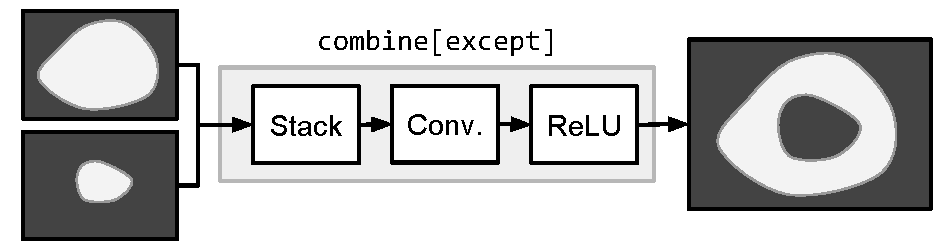
\includegraphics[width=\columnwidth]{fig/combine}

\paragraph{Classify}

A classification module \mod{classify[$x$]} takes an attention and the input
image and maps them to a distribution over labels. For example, {\small\tt
classify[color]} should return a distribution over colors for the region
attended to.\\[1em]
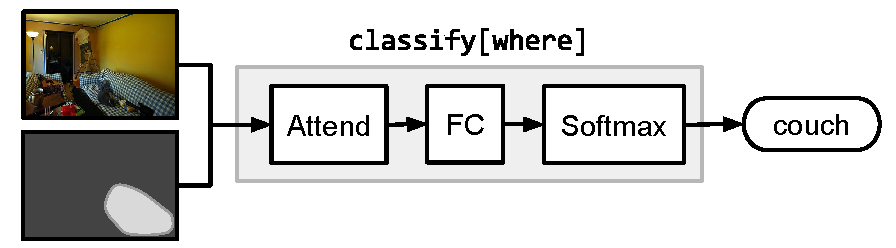
\includegraphics[width=\columnwidth]{fig/classify}

\subsection{From strings to networks}

In this section, we first describe how to map from natural language questions to
\emph{layouts}, which specify both the set of modules used to answer a given
question, and the connections between them. Next we describe how layouts are
used to assemble the final prediction networks.

To predict layouts use standard tools pre-trained on existing linguistic
resources to obtained structured representations of questions. Future work might
focus on learning (or at least fine-tuning) this prediction process jointly with
the rest of the system, though in fact off-the-shelf tools produce high-quality
analyses for almost all the questions in our data.

Specifically, we begin by parsing each question with the Stanford Parser (XXX)
to obtain a universal dependency representation (XXX). Dependency parses express
grammatical relations between parts of a sentence (e.g.\ between objects and
their attributes, or events and their participants), and provide a lightweight
abstraction away from the surface form of the sentence.

Next, we filter the set of dependencies to those involving the wh-word in the
question (XXX and more). This gives a simple logical form expressing (the
primary) part of the sentences meaning. For example, \emph{what is standing in
the field} becomes \mod{what(stand)}; \emph{what color is the truck} becomes
\mod{color(truck)}, and \emph{is there a circle next to a square} becomes
\mod{is(cicle, next-to(square))}. The code for peforming this transformation is
simple, and provided in the accompanying software distribution.

XXX something about combinator logics / leaves of the tree.

These logical forms already determine the structure of the predicted network,
but not the identities of the modules that compose it. This final assignment of
modules is fully determined by the structure of the parse. All leaves become
\mod{attend} modules, all internal nodes become \mod{re-attend} or \mod{combine}
modules dependint on their arity, and root nodes become \mod{classify} modules.

Given the mapping from queries to network layouts described above, we have for
each training example a network structure, an input image, and an output label.
In many cases, these network structures are different, but have tied parameters.
Networks which have the same high-level structure but different instantiations
of individual modules (for example \emph{what color is the cat}---{\small\tt
classify[color](detect[cat])} and \emph{where is the truck}---{\small\tt
classify[where](detect[truck])}) can be processed in the same batch, resulting
in efficient computation.


\begin{figure*}
    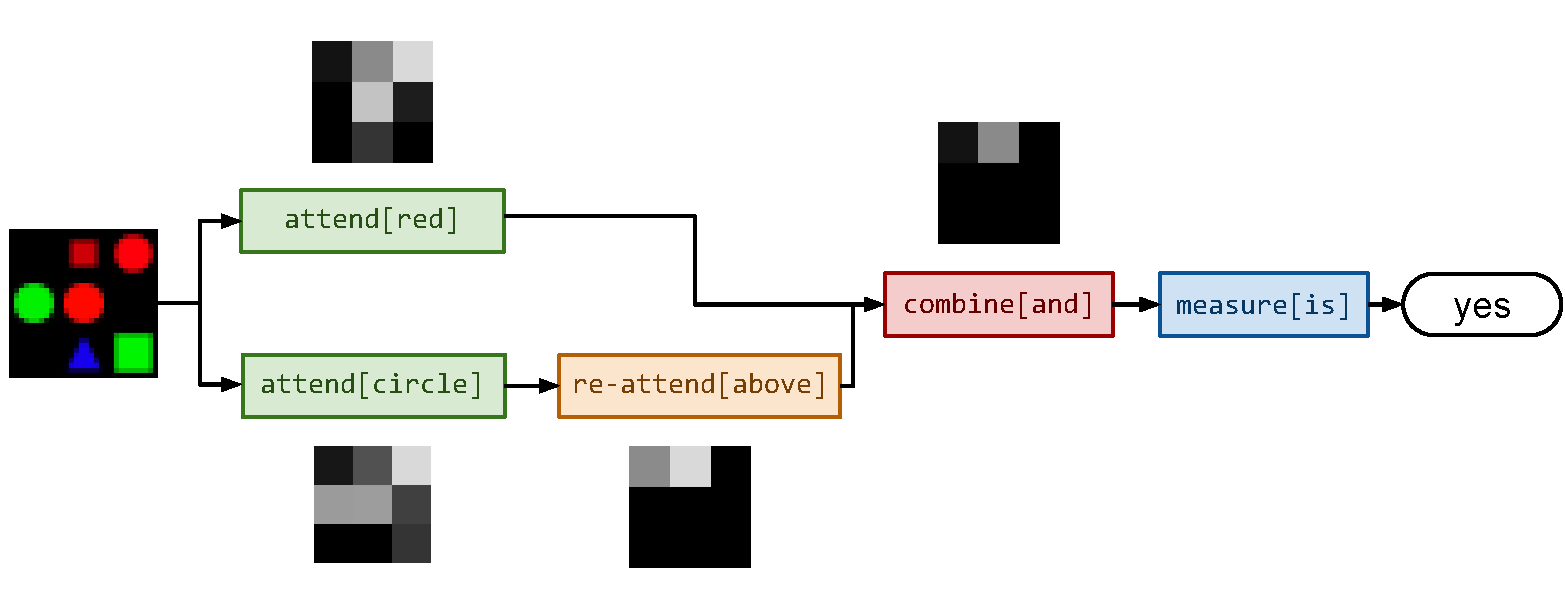
\includegraphics[width=\textwidth]{fig/full2}
\end{figure*}

\section{Learning}

Our training objective is simply to find module parameters maximizing the
likelihood of the data. By design, the last module in every network is a
{\small\tt classify}, and so each assembled network represents a probability
distribution.

Because of the dynamic network structures used to answer questions, some weights
are updated much more frequently than others. For this reason we found that
learning algorithms with adaptive per-weight learning rates performed
substantially better than simple gradient descent. All the experiments described
below use AdaDelta (XXX) (thus there was no hyperparameter search over step sizes).

It is important to emphasize that the labels we have assigned to distinguish
instances of the same module type---\mod{cat}, \mod{and}, etc.---are a
notational convenience, and do not reflect any manual specification of the
behavior of the corresponding modules. \mod{detect[cat]} doesn't know it's
supposed to be a cat detector (rather than a couch detector or a dog detector),
and \mod{combine[and]} doesn't know it's supposed to compute intersections of
attentions (rather than unions or differences). Instead, they acquire these
semantics as a byproduct of the end-to-end training procedure. As can be seen in
Figure XXX, the image--answer pairs and parameter tying together encourage each
module to specialize in the appropriate way.

%---a simple feedforward
%convolutional network is suitable for most detection and classification tasks,
%but counting to arbitrary numbers probably requires a recurrent network.

\section{Experiments: natural images}

For both experiments in this section, the input to each \mod{attend} module is
the the Conv XXX layer of an Oxford VGGNet (XXX) after max-pooling. We do not
fine-tune the VGGNet.

\begin{table}
  \footnotesize
  \center
  \begin{tabular}{cccccc}
    \toprule
    System & All & Yes/No & Color & Number & Other \\
    \midrule
    IMG+BOW & 55.92 & 58.66 & 49.39 & 51.96 & 44.10 \\
    2-VIS+BLSTM & 55.09 & 58.17 & 47.34 & 49.53 & 44.79 \\
    NMN (indep) \\
    NMN \\
    \bottomrule
  \end{tabular}
  \caption{CocoQA results}
\end{table}

\begin{table}
  \footnotesize
  \center
  \begin{tabular}{cccccc}
    \toprule
    System & All & Object & Location & Color & Number \\
    \midrule
    VIS+LSTM & 53.74 & 78.94 & 43.53 & 36.42 & \\
    NMN \\
    \bottomrule
  \end{tabular}
  \caption{VQA results}
\end{table}


\section{Experiments: compositionality}

Past work [Ren paper] has achieved state-of-the-art results on the CocoQA
dataset using a bag-of-words model . This is consistent with [VQA paper]'s
observation that image features are most important for simple object- and
activity-recognition questions, and that they make little difference for other
categories (like yes/no questions). Taken together, these results suggest that
existing natural image datasets primarily require simple object- and attribute
detection, with limited importance attached to spatial relations and other
highly compositional phenomena.

As one of the primary goals of this work is to learn models for deep semantic
compositionality, we have created an additional dataset that places such
compositional phenomena at the forefront. This dataset consists of highly
structured questions about simple arrangements of colored shapes [XXX].
Questions contain between two and four attributes, object types, or
relationships.  There are 244 questions and 15616 images in total, divided into
train and test sets (with no overlap between the train and test sets).  To
eliminate mode-guessing as a viable strategy, all questions have a yes-or-no
answer, but good performance requires that the system learn to recognize shapes
and colors, and understand both spatial and logical relations among sets of
objects.

XXX babyai

\begin{figure}
  \centering
  \emph{Is there a red shape above a circle?} \\[1em]
  \begin{tabular}{ccc}
    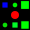
\includegraphics[width=0.25\columnwidth]{fig/shapes1} &
    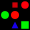
\includegraphics[width=0.25\columnwidth]{fig/shapes2} &
    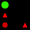
\includegraphics[width=0.25\columnwidth]{fig/shapes3} \\
    no & yes & yes
  \end{tabular}
  \caption{Example question, images, and answers from the \shapes dataset.
    Answering this question requires being able to recognize an object
    (\emph{circle}), an attribute (\emph{red}), and a spatial relation
    (\emph{above}), and compare sets of objects having all these properties.}
\end{figure}


\begin{table}
  \footnotesize
  \center
  \begin{tabular}{ccccc}
    \toprule
    System & All & Size 2 & Size 3 & Size 4 \\
    \midrule
    IMG+BOW & \\
    VIS+LSTM &  \\
    NMN & 90.62* & 89.69* & 92.36* & 85.16* \\
    \bottomrule
  \end{tabular}
  \caption{Synth data results}
\end{table}

As can be seen, our model achieves excellent performance on this dataset, while
competing approaches fare little better than the majority baseline. Moreover,
the color detectors and attention transformations behave as expected, indicating
that our joint training procedure correctly allocates responsibilities among
modules. Ultimately, in addition to achieving competitive results in answering
simple questions about natural images, our approach is able to model complex
compositional phenomena outside the capacity of previous approaches to visual
question answering.

\section{Conclusions and future work}

In this paper, we have introduced \emph{neural module networks}, which provide a
general-purpose framework for learning collections of neural modules which can
be dynamically assembled into arbitrary deep networks. We have demonstrated that
this approach achieves state-of-the-art performance on existing datasets for
visual question answering. Additionally, we have introduced a new dataset of
highly compositional questions about simple arrangements of shapes, and shown
that our approach substantially outperforms previous work.

So far we have maintained a strict separation between predicting network
structures and learning network parameters. It is easy to imagine that these two
problems might be solved jointly, with uncertainty maintained over network
structures throughout training and decoding. This might be accomplished either
XXX.

The fact that deep neural modules can be trained to produce predictable
outputs---even when freely composed---points toward a more general paradigm of
``programs'' built from neural networks. In this paradigm, network designers
(human or automated) have access to a standard kit of neural parts from which to
construct models for performing complex reasoning tasks. While visual question
answering provides a natural testbed for this approach, its usefulness is
potentially much broader, extending to queries about documents and structured
knowledge bases or more general signal processing and function approximation.

\small
\bibliographystyle{ieee}
\bibliography{biblioShort,rohrbach,related,jacob}


\end{document}
